%!TEX TS-program = xelatex
%!TEX encoding = UTF-8 Unicode
\documentclass{beamer}
\usetheme{CambridgeUS} % replace it with Boadilla if you want no section bar
%\usecolortheme{crane} % other ones: dove, dolphin, rose, seahorse, orchid, crane, seagull, lily, wolverine
%\usefonttheme{serif} 
\usefonttheme[onlymath]{serif} % uncomment if you want it just for math

\setbeamertemplate{navigation symbols}{}  % comment to have nagivation

\usepackage[compress,comma,authoryear]{natbib}
\usepackage{tikz}
\usetikzlibrary{mindmap,trees}
\usepackage{amsmath,mathtools}
\usepackage{amsthm}
\usepackage{booktabs}
\usepackage{graphicx,epstopdf}
\usepackage{hyperref}
\usepackage{fontspec}
\newfontfamily{\FA}{XB Niloofar}[Extension = .ttf] % Farsi
\newfontfamily{\FAN}{IranNastaliq}[Extension = .ttf] % Farsi Nastaliq

\definecolor{blue}{RGB}{0,114,178}
\definecolor{red}{RGB}{213,94,0}
\definecolor{yellow}{RGB}{240,228,66}
\definecolor{green}{RGB}{0,158,115}
\definecolor{Lblue}{RGB}{0,197,155}
\definecolor{Dblue}{RGB}{0,76,119}
\definecolor{Lgreen}{RGB}{180,255,230}

\hypersetup{
	colorlinks=false,
	linkbordercolor = {white},
	linkcolor = {blue}
}
\definecolor{MyBackground}{RGB}{245,245,245}

\setbeamercolor{frametitle}{fg=blue}
\setbeamercolor{title}{fg=blue}
\setbeamertemplate{footline}[frame number]
\setbeamertemplate{navigation symbols}{} 
\setbeamertemplate{itemize item}[circle]%{$\bigstar$}
\setbeamertemplate{itemize subitem}{$\bigstar$}
\setbeamercolor{itemize item}{fg=blue}
\setbeamercolor{itemize subitem}{fg=blue}
\setbeamercolor{enumerate item}{fg=blue}
\setbeamercolor{enumerate subitem}{fg=blue}
\setbeamercolor{button}{bg=MyBackground,fg=blue}
\setbeamercolor*{palette primary}{use=structure,fg=blue,bg=white}
\setbeamercolor*{palette secondary}{use=structure,fg=white,bg=Dblue}
\setbeamercolor*{palette tertiary}{use=structure,fg=white,bg=blue}
\setbeamercolor*{palette quaternary}{fg=white,bg=black}
\setbeamercolor*{palettes quaternary}{fg=white,bg=Lgreen}
%\setbeamercolor{titlelike}{parent=structure,bg=Lgreen}
%\setbeamercolor{title in head/foot}{bg=Lgreen,fg=orange}

\setbeamertemplate{enumerate item}{%
	\usebeamercolor[bg]{item projected}%
	\raisebox{1.5pt}{\colorbox{blue}{\color{fg}\footnotesize\insertenumlabel}}%
}





\begin{document}
	\title[Econometrics 2]{Econometrics 2 (M.Sc.)}
	\subtitle{Basic Regression Talks}
	\author[Mohammad Hoseini]{Mohammad Hoseini}
	
	%\institute[IMPS]{Institute for Management and Planning Studies (IMPS)}
	
	\date[Spring 2024]{Spring 2024 \\
	\vspace{10pt} @metrics2
}

	
\begin{frame}[plain]
	\titlepage
\end{frame}

\section{Regression}
\subsection{OLS}
\begin{frame}{Ordinary Least Square (OLS)}
Minimizing the sum of the squares of the differences between the observed dependent variable and those predicted by the linear function.

\[y_i=bX_i+\varepsilon_i \ \Rightarrow \ \beta=\arg\min_b E[(y_i-bX_i)^2] \]
\[\text{FOC: }\ E[X_i(y_i-bX_i)]=0 \ \Rightarrow \ \beta=E[X_iX_i']^{-1}E[X_iY_i] \]


\end{frame}




\begin{frame}{Bivariate case}

\[y_i=\alpha+\beta x_i+\varepsilon_i\]
\[\arg\min_{\alpha,\beta} E[(y_i-\alpha-\beta x_i)^2] =\arg\min_{\alpha,\beta} \frac{1}{n}\sum_{i=1}^n(y_i-\alpha-\beta x_i)^2 \]\pause
FOC: 
\begin{enumerate}
\item $-2E[y_i-\alpha-\beta x_i]=0\ \Rightarrow \ \alpha=\bar{y}-\beta \bar{x} $
\item $-2E[x_i(y_i-\alpha-\beta x_i)]=0\ \Rightarrow \ \frac{1}{n}\sum_i x_iy_i =\alpha\bar{x}+\beta\frac{1}{n}\sum_i x_i^2 $
\end{enumerate} 

\[\beta=\frac{\sum_i(y_i-\bar{y})(x_i-\bar{x})}{\sum_i(x_i-\bar{x})^2}=\frac{\text{COV}(y_i,x_i)}{\text{VAR}(x_i)} \ ,\quad \alpha=\bar{y}-\beta\bar{x} \]
Note that $0\le \text{Corr}(x,y)=\beta\frac{\sigma_x}{\sigma_y}\le1$. This helps in scaling coefficient and interpretation. 

\end{frame}


\begin{frame}{Illustration of linear regression $y_i=\alpha+\beta x_i+\varepsilon_i$}

\begin{columns}
\begin{column}{0.65\linewidth}
\[	\beta_i=\frac{y_i-\bar{y}}{x_i-\bar{x}}, \quad \beta_j=\frac{y_j-\bar{y}}{x_j-\bar{x}}\]
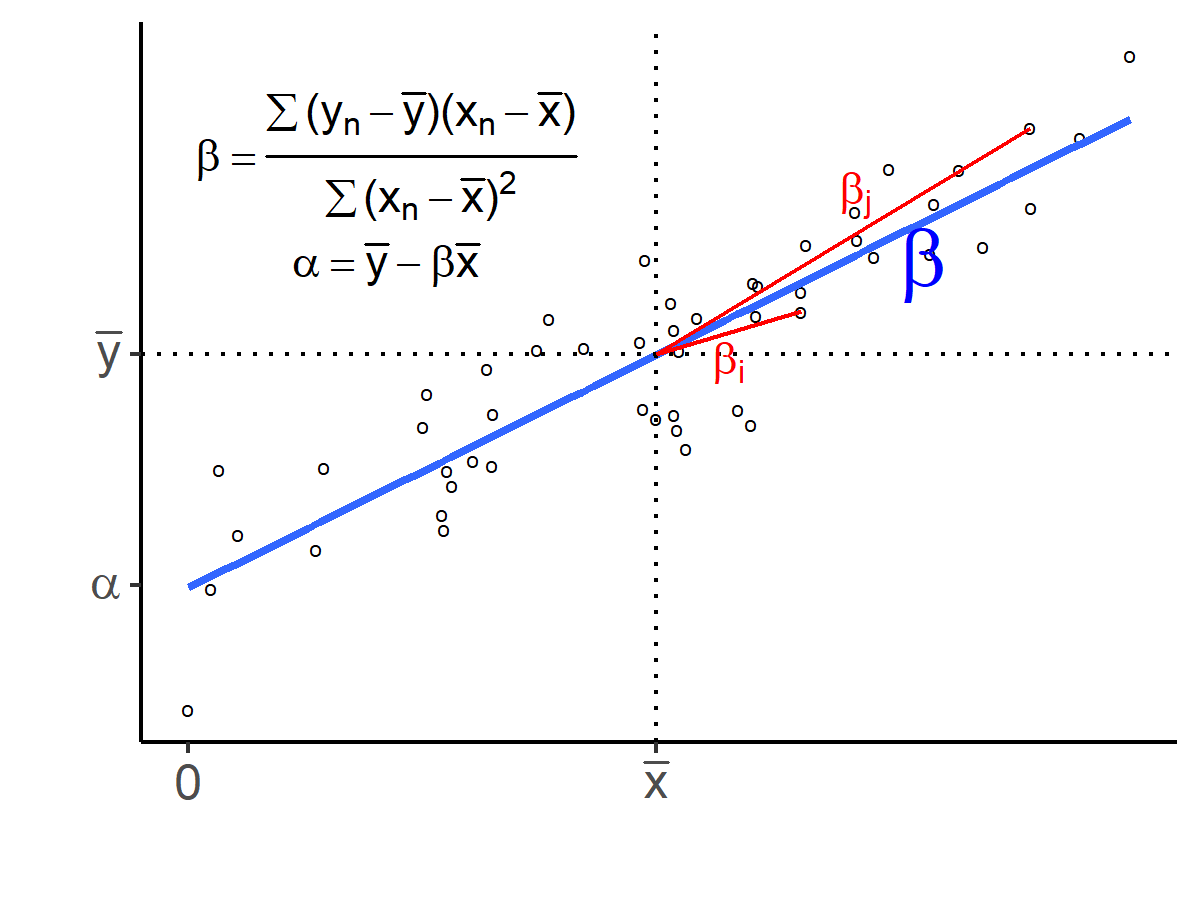
\includegraphics[width=.95\linewidth]{./Figures/plot.png}
\end{column}
\begin{column}{0.35\linewidth}
\[\beta=g(\beta_1,\dots,\beta_n) \] \pause
If error terms are normally distributed:	\[\beta=\sum_{k=1}^N \gamma_k \beta_k\]
\[\gamma_k=\frac{(x_k-\bar{x})^2}{\sum_{s=1}^N(x_s-\bar{x})^2} \]	
Observations further from the mean of $x$ have higher signal to noise ratio and get higher weights.


\end{column}

\end{columns}

\end{frame}

\begin{frame}{STATA example}

\begin{tt}
clear all \medskip

set obs 100  \qquad {\color{teal} // setting the number of observations}\medskip

generate x=rnormal(2,1) \qquad {\color{teal} // $x \sim \textit{N}(2,1)$}\medskip

generate e=rnormal() \qquad {\color{teal} // $\varepsilon \sim \textit{N}(0,1)$}\medskip

generate y=1+x+e \qquad {\color{teal} // $y=1+x+\varepsilon, \  $}\medskip

summarize x e y \medskip

regress y x \medskip

twoway scatter y x || lfit y x \medskip
\end{tt}
\end{frame}

\begin{frame}{Regression anatomy}
Bivariate case $y_i=\beta_0+\beta_1x_i+\varepsilon_i \ \Rightarrow \ \beta_1=\frac{\text{COV}(y,x)}{\text{VAR}(x)}$\bigskip\pause

Multivariate case: $y_i=\beta_0+\beta_1 x_{1i}+\beta_2 x_{2i}+\dots+\beta_n x_{ni}+\varepsilon_i$\medskip\pause

Let $x_{ki}=\delta_0+\delta_1 x_{1i}+\dots+\delta_{k-1}x_{k-1 i}+\delta_{k+1}x_{k+1i}+\dots+\beta_nx_{ni}+\epsilon_i$ and $\tilde{x}_{ki}=x_{ki}-\hat{x}_{ki}$\pause

\[ \beta_k=\frac{\text{COV}(y,\tilde{x})}{\text{VAR}(\tilde{x})} \]

\begin{itemize}
\item $\tilde{x}_i$ is the residual from a regression of $x_{ki}$ on all other covariates.
\end{itemize}
Each coefficient in a multivariate regression is the bivariate slope coefficient for the corresponding regressors, after ``partialling out'' all other variables in the model.

\end{frame}



\begin{frame}{STATA example}

\begin{tt}
sysuse auto, clear
\qquad {\color{teal} // a default dataset of STATA}\medskip

describe\medskip

regress price length  \qquad {\color{teal} // bivariate regression}\medskip

regress price length mpg weight  {\color{teal} // multivariate regression}\medskip

regress length mpg weight\medskip

predict reslengthr, r {\color{teal} // partialling out  other covariates}\medskip

regress price reslength\medskip

twoway scatter price length || lfit price length\medskip

twoway scatter price reslength || lfit price reslength 

\end{tt}
\end{frame}

\begin{frame}{Graph data before running regressions} 
\begin{columns}
\begin{column}{0.4\linewidth}
For all graphs:
\begin{itemize}
\item $\bar{x}=9$	
\item $\sigma^2_x=11$
\item $\bar{y}=7.50$
\item $\sigma^2_y=4.125$
\item $\text{Corr}_{x,y}=0.816$
\item regression line $y=3.00+0.500x$
\item $R^2= 0.67$
\end{itemize}
\end{column}
\begin{column}{0.6\linewidth}
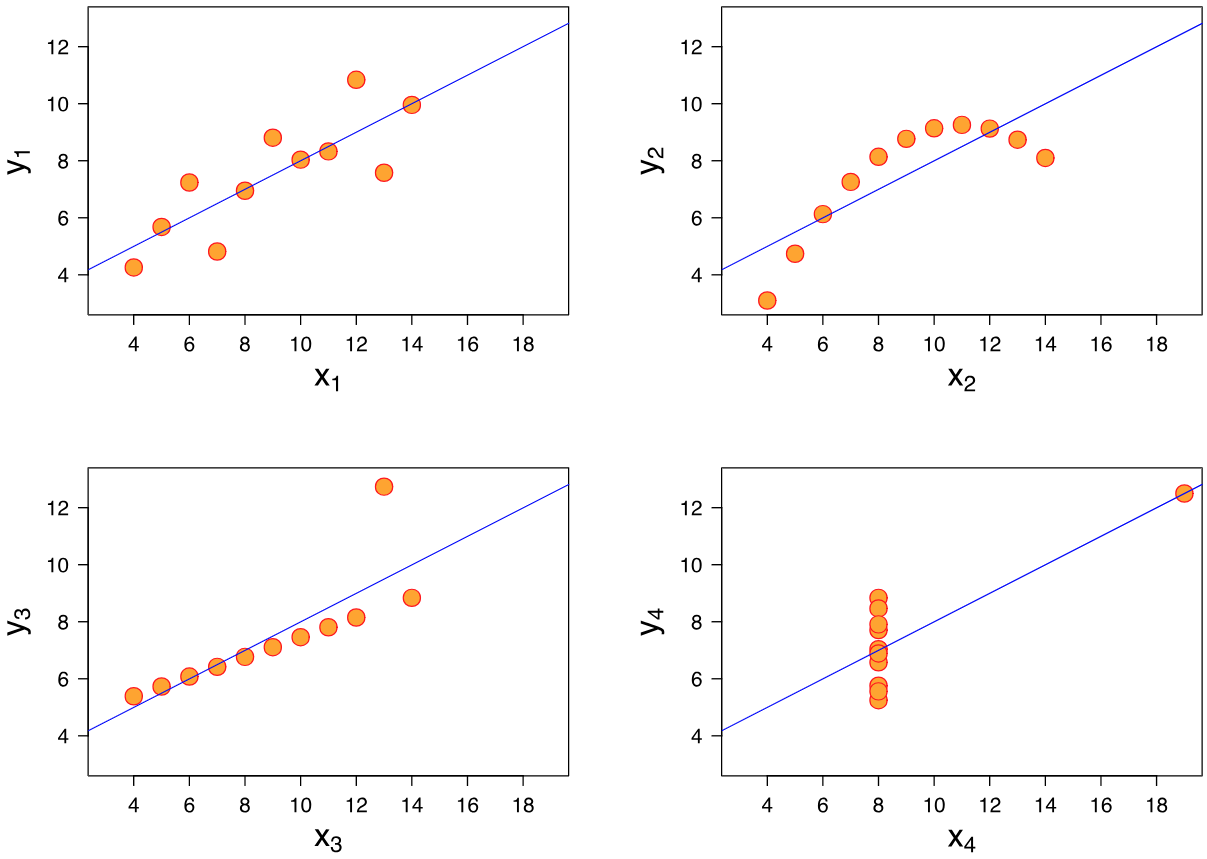
\includegraphics[width=\linewidth]{./Figures/Anscombe}
\end{column}
\end{columns}\pause
Graphing regression anatomy can simply show whether outliers drive the results or not.




\end{frame}

\begin{frame}{Interpretation of regression in the past and present}
Empirical micro papers 30 years ago (probabilistic causality):
\begin{itemize}
\item A regression motivated by a complex model and the equation meant to describe an economic process
\item All regressors on the RHS were more or less equally important.
\end{itemize}\bigskip

Empirical micro papers nowadays (counter-factualist causality):
\begin{itemize}
\item Focusing on one causal relationship 
\item Identification strategy meant to eliminate selection bias
\item Regressors are not equally important and only one variable is seen as having causal effects.
\item All others are controls included in service of the focused causal agenda.

\end{itemize}

\end{frame}



\subsection{Some common regressions}

\begin{frame}{Saturated models}
Suppose we want to estimate the effect of years of schooling on income:
\begin{itemize}
\item We can estimate $y_i$ on years of schooling $D_i=0,1,\dots, 12$   \[y_i=\alpha+\beta D_i+X_i'\gamma +e_i \]\pause
\item We can estimate a saturated model with year dummies $d_{ji}=1(D_i=j)$
\[y_i=\beta_0+\beta_1 d_{1i}+\beta_2 d_{2i}+\dots+\beta_{12} d_{12i}+X_i'\gamma +e_i \]
\end{itemize}
j-th year effect of schooling: $E[y_i|D_i=j]-E[y_i|D_i=0]=\beta_j$.

\end{frame}

\begin{frame}{Main effect and interaction term}
Suppose we want to estimate the effect of school attendence ($x_1$) and gender ($x_2$) on adult income ($y$).
\[y_i=\alpha+\beta_1 x_{1i}+\beta_2 x_{2i}+\beta_3 x_{1i}x_{2i}+e_i \]
\begin{itemize}
\item $E[y_i|x_{1i}=0,x_{2i}=0]=\alpha $
\item $E[y_i|x_{1i}=1,x_{2i}=0]=\alpha+\beta_1 $
\item $E[y_i|x_{1i}=0,x_{2i}=1]=\alpha+\beta_2 $
\item $E[y_i|x_{1i}=1,x_{2i}=1]=\alpha+\beta_1+\beta_2+\beta_3 $
\end{itemize}\medskip\pause

The saturated model with years of schooling
\[y_i=\beta_0+\sum_{j=1}^{12} \beta_j d_{ji}+\delta x_{2i}+\sum_{j=1}^{12}\gamma_j d_{ji}\times x_{2i} \]
\end{frame}


\begin{frame}{Principle of marginality}
If an interaction is on RHS, all main effects should also be there.
\begin{figure}
\centering
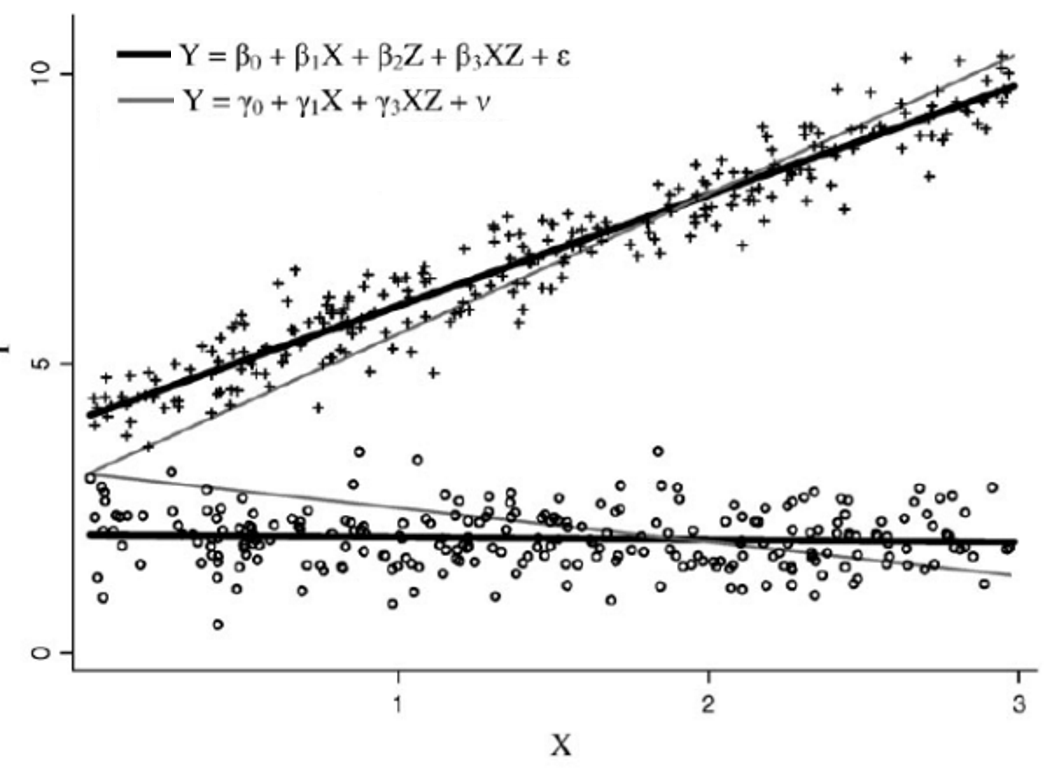
\includegraphics[width=0.68\linewidth]{./Figures/principleofmarginality}
\label{fig:principleofmarginality}
\end{figure}

\end{frame}
\begin{frame}{Interaction term as an exaggerator}
Does resource abundance cause growth? \citep{mehlum2006institutions}
\begin{columns}
	\begin{column}{.7\textwidth}
  \quad	\includegraphics[width=.9\linewidth]{./Figures/resourcecurse.png}%\pause
	\end{column}
	\begin{column}{.3\textwidth}
		\begin{center}
    \FAN{\LARGE می‌کند \ شر \ سری \ هر \ در \ نی \ باده
    	
    	{\color{red} 
    	می‌کند \ \ آن‌چنان‌تر \ \ را \ \ آن‌چنان‌
    	}\vspace{.5cm}
    	
    	می‌شود \ نکوفر \ عاقل \ خورد \ گر
    	\vspace{5pt}
    	
    	می‌شود \ بدتر \ بدخوی \ \ خورد \ ور
    }\end{center}
    \end{column}
\end{columns}

%\begin{figure}
%	\centering
%	\includegraphics[width=0.5\linewidth]{../figure/resourcecurse}%\pause
%		\includegraphics[width=0.45\linewidth]{../figure/interactionterm}
%	\end{figure}
\end{frame}

\begin{frame}{Weighting regressions}
In many household or firm-level surveys, samples have weight, i.e. how many household/firm they represent. 
\bigskip

Or we may have data grouped at level $s$, such that %province level
in each $s$ we have random sample with $\bar{y}_s=E[y_i|s_i=s]$.\bigskip

We also know relative frequency of $s$: $n_s/N$. The regression of $\bar{y}_s$ on $s$ weighted by $n_s$ is the same as a random-sample regression.
\bigskip

In cases like these we need to run weighted regression in STATA:

{\texttt{. regress y x [weight=W]} } 
\end{frame}

\subsection{Standard error issues}

\begin{frame}{Standard errors in regressions}
The standard errors determine how significant is the estimation and how many stars you get in the tables.\bigskip

The correct SE estimation depends on the structure of the data.\bigskip

In basic regression, we assume the error terms are independent and identically distributed (i.i.d)\bigskip

This assumption can be violated in many instances:
\begin{itemize}
\item The variance of income is often higher in families with higher income (heteroskedasticity)
\item In the panel data, the error-terms for one individual are usually correlated.
\end{itemize}

\end{frame}


\begin{frame}{Homoskedastic case (i.i.d)}
\[ y_i=\beta_0+\beta_1x_i+\varepsilon_i,\qquad \varepsilon_i\sim (0,\sigma^2) \]
Then \[E\{\varepsilon\varepsilon'\}=E\left\{ \left[\begin{array}{c}
\varepsilon_1 \\
\vdots \\
\varepsilon_n
\end{array} \right] \times [\varepsilon_1,  \dots , \varepsilon_n]\right\}= \left[\begin{array}{cccc}
\sigma^2 & 0& \dots & 0\\
0 & \sigma^2 &\dots& 0\\
\vdots & \vdots & &\vdots \\
0&0 &\dots&\sigma^2
\end{array} \right]=\sigma^2I_n\]

\[\hat{\beta}_1=\frac{\sum_i (x_i-\bar{x})(y_i-\bar{y})}{\sum_i(x_i-\bar{x})^2} , \quad\hat{\sigma}^2=\frac{\sum_i(y_i-\hat{\beta}_0-\hat{\beta}_1{x}_i)^2}{n-2} \]
%\[ \hat{\beta}_1-\beta_1=\frac{\sum_i (x_i-\bar{x})\varepsilon_i}{\sum_i(x_i-\bar{x})^2}, \ \text{VAR}(\hat{\beta})=\frac{\sigma^2}{\sum_i(x_i-\bar{x})^2} \]
\[ \text{SE}(\hat{\beta})=\frac{\hat{\sigma}}{\sqrt{\sum_i(x_i-\bar{x})^2}} \ , \quad  \frac{\hat{\beta}-\beta}{\text{SE}(\hat{\beta})}\sim \text{t-student}(n-2) \]
\end{frame}

\begin{frame}{Heteroskedastic case (i.n.i.d)}
\[ y_i=\beta_0+\beta_1x_i+\varepsilon_i,\qquad \varepsilon_i\sim (0,\sigma^2_i) \]
Then \[E\{\varepsilon\varepsilon'\}=E\left\{ \left[\begin{array}{c}
\varepsilon_1 \\
\vdots \\
\varepsilon_n
\end{array} \right] \times [\varepsilon_1,  \dots , \varepsilon_n]\right\}= \left[\begin{array}{cccc}
\sigma^2_1 & 0& \dots & 0\\
0 & \sigma^2_2 &\dots& 0\\
\vdots & \vdots & &\vdots \\
0&0 &\dots&\sigma^2_n
\end{array} \right]=\Omega \]
In this case the previous formula for $SE(\hat{\beta})$ is not valid.
\end{frame}


\begin{frame}{Clustered cases (n.i.n.i.d)}
Clustered data with $m$ clusters 
\footnotesize 
$E\{\varepsilon\varepsilon'\}=$ \[\left[\begin{matrix}
\sigma^2_{(11)1} & \dots & \sigma^2_{(1n_1)1}&0&\dots&0&\dots&0& \dots & 0\\
\vdots & \ddots & \vdots&\vdots & \ddots & \vdots&\ddots&\vdots & \ddots & \vdots\\
\sigma^2_{(n_11)1} & \dots & \sigma^2_{(n_1n_1)1}&0&\dots&0&\dots&0& \dots & 0\\
0&\dots&0&\sigma^2_{(11)2} & \dots & \sigma^2_{(1n_2)2}&\dots&0& \dots & 0\\
\vdots & \ddots & \vdots&\vdots & \ddots & \vdots&\ddots&\vdots & \ddots & \vdots\\
0&\dots&0&\sigma^2_{(n_21)2} & \dots & \sigma^2_{(n_2n_2)2}&\dots&0& \dots & 0\\
\vdots&&\vdots&\vdots&&\vdots&\ddots&\vdots&&\vdots\\
0&\dots&0&0& \dots & 0&\dots&\sigma^2_{(11)m} & \dots & \sigma^2_{(1n_m)m}\\
\vdots & \ddots & \vdots&\vdots & \ddots & \vdots&\ddots&\vdots & \ddots & \vdots\\
0&\dots&0&0& \dots & 0&\dots&\sigma^2_{(n_m1)m} & \dots & \sigma^2_{(n_mn_m)m}\\
\end{matrix} \right] \]
\end{frame}

\begin{frame}{General case (n.i.n.i.d)}
\[E\{\varepsilon\varepsilon'\}=E\left\{ \left[\begin{array}{c}
\varepsilon_1 \\
\vdots \\
\varepsilon_n
\end{array} \right] \times [\varepsilon_1,  \dots , \varepsilon_n]\right\}= \left[\begin{array}{cccc}
\sigma^2_1 & \sigma^2_{12}& \dots & \sigma^2_{1n}\\
\sigma^2_{21} & \sigma^2_2 &\dots& \sigma^2_{2n}\\
\vdots & \vdots & \ddots&\vdots \\
\sigma^2_{n1}&\sigma^2_{n2} &\dots&\sigma^2_n
\end{array} \right] \]

\end{frame}



\begin{frame}{Robust standard errors}

Heteroskedasticity: VAR($\varepsilon_i)=\sigma_i^2,\ \sigma_i\neq\sigma_j$\\
Homoskedasticity $\forall i,$  VAR($\varepsilon_i)=\sigma^2$\medskip

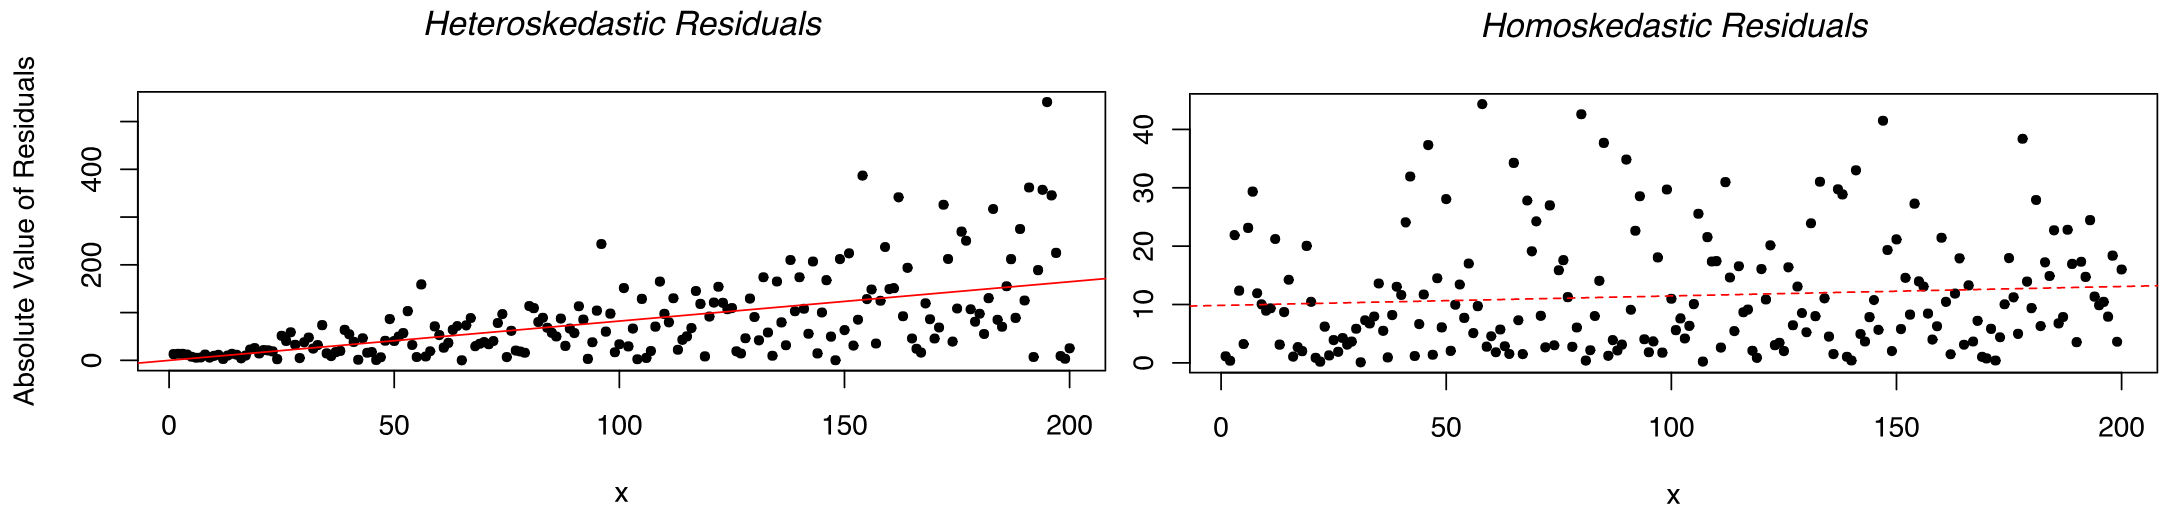
\includegraphics[width=1\linewidth]{./Figures/robust}

To solve heteroskedasticity in STATA: \texttt{ regress y x, robust}\bigskip

Note that using robust SEs are not always better. Only when heteroskedasticity is large it works better than non-robust.\medskip

A rule of thumb: take the max of robust and non-robust SEs.
\end{frame}


\begin{frame}{Clustered standard error}
When observations are correlated within certain groups we use clustering.\bigskip

Example: The effect of class size on students' grades. \medskip

The unobservable variables of students in the same class are correlated (teacher, peer effect, etc.) while it is not correlated with students of other classes.\bigskip

We should cluster SEs based on classroom.\bigskip

In STATA:  \quad \texttt{regress grade size, cluster(classroom)}\bigskip

Clustering SE increases the resulting SEs and we get less star in the tables.\bigskip

See \cite{abadie2023should} for the level of clustering.
\end{frame}

\begin{frame}{FGLS}
In more general cases, we can use Feasible Generalized Least Square (FGLS).\medskip

Note that GLS is more efficient than OLS under heteroscedasticity or autocorrelation, this is not true for FGLS.\medskip

FGLS estimates the covariance matrix $\Omega$ at step 1 and uses it to find coefficients at stage 2: $\hat{\beta}=\arg\min (y-X\beta)'\Omega^{-1}(y-X\beta)$.\bigskip

Therefore, in FGLS the $\hat{\beta}$ changes compared to OLS. \medskip

Use of robust or clustered covariance matrix, however, leaves $\hat{\beta}$ the same as OLS, but attempts to fix confidence intervals.\medskip

Based on the covariance structure using FGLS can be superior or inferior.\medskip

In small sample FGLS are normally less efficient than clustering. \medskip %and in large sample cross-correlation is only important within some clusters.

In micro panel data, FGLS is used to estimate random effect models.

\end{frame}

\begin{frame}{All depends on the your data}
You need to know your data in order to choose correct error structure and then infer the SE specification. \bigskip

In real world, i.i.d is normally violated, but using more complex structure also sacrifices efficiency.\bigskip

Graphing the error-term or heteroskedasticity tests can also help to choose the kind of SE specification\bigskip

If the data has some level of aggregation (like classroom, province, state, etc.) clustering is important.\bigskip

In difference-in-difference estimations with multiple time spots clustering is required.\medskip



\end{frame}



\begin{frame}{References:}
\bibliographystyle{apalike}
\small
\bibliography{./references}
\end{frame}

\end{document}
